% =============================================================================
% Cycle de vie d'un ticket — diagrammes d'activité
% TicketManager — formulation académique
% Figures : docs/release-1/img/cycle-vie-ticket-*.png
% =============================================================================

\subsection{Cycle de vie d'un ticket}

Un ticket traverse quatre statuts successifs : \textbf{Ouvert}, \textbf{En cours},
\textbf{Résolu} et \textbf{Clôturé}. La figure~\ref{fig:cycle-vie-general}
présente la vue d'ensemble du cycle ; la
figure~\ref{fig:cycle-vie-detaille} en détaille les activités par acteur et
les interactions avec la plateforme.

\begin{figure}[htbp]
    \centering
    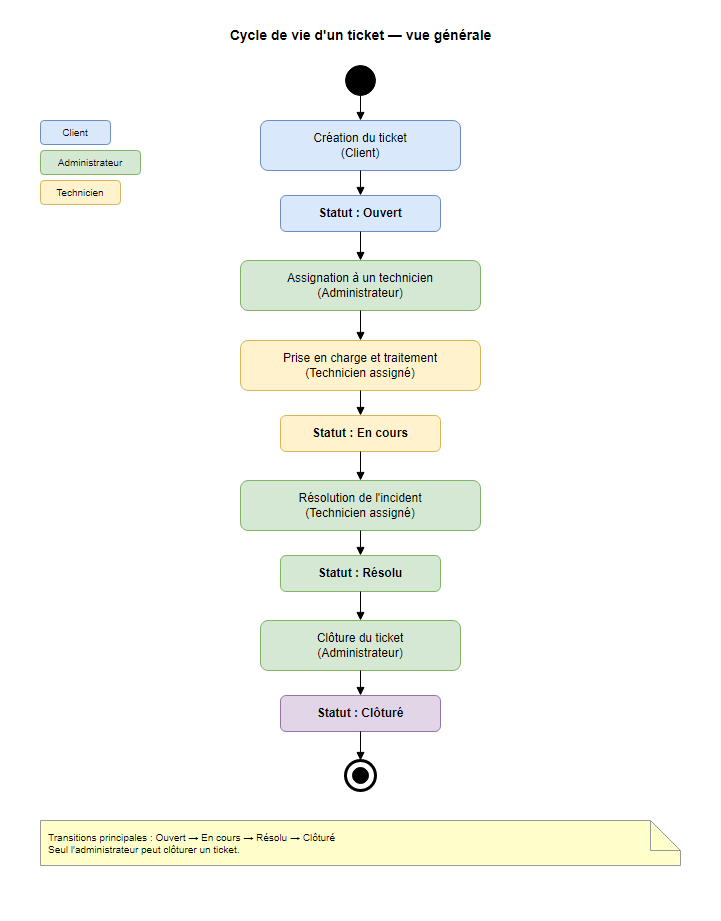
\includegraphics[width=0.72\textwidth]{img/cycle-vie-ticket-general.png}
    \caption{Cycle de vie d'un ticket — vue générale (création à clôture)}
    \label{fig:cycle-vie-general}
\end{figure}

\begin{figure}[htbp]
    \centering
    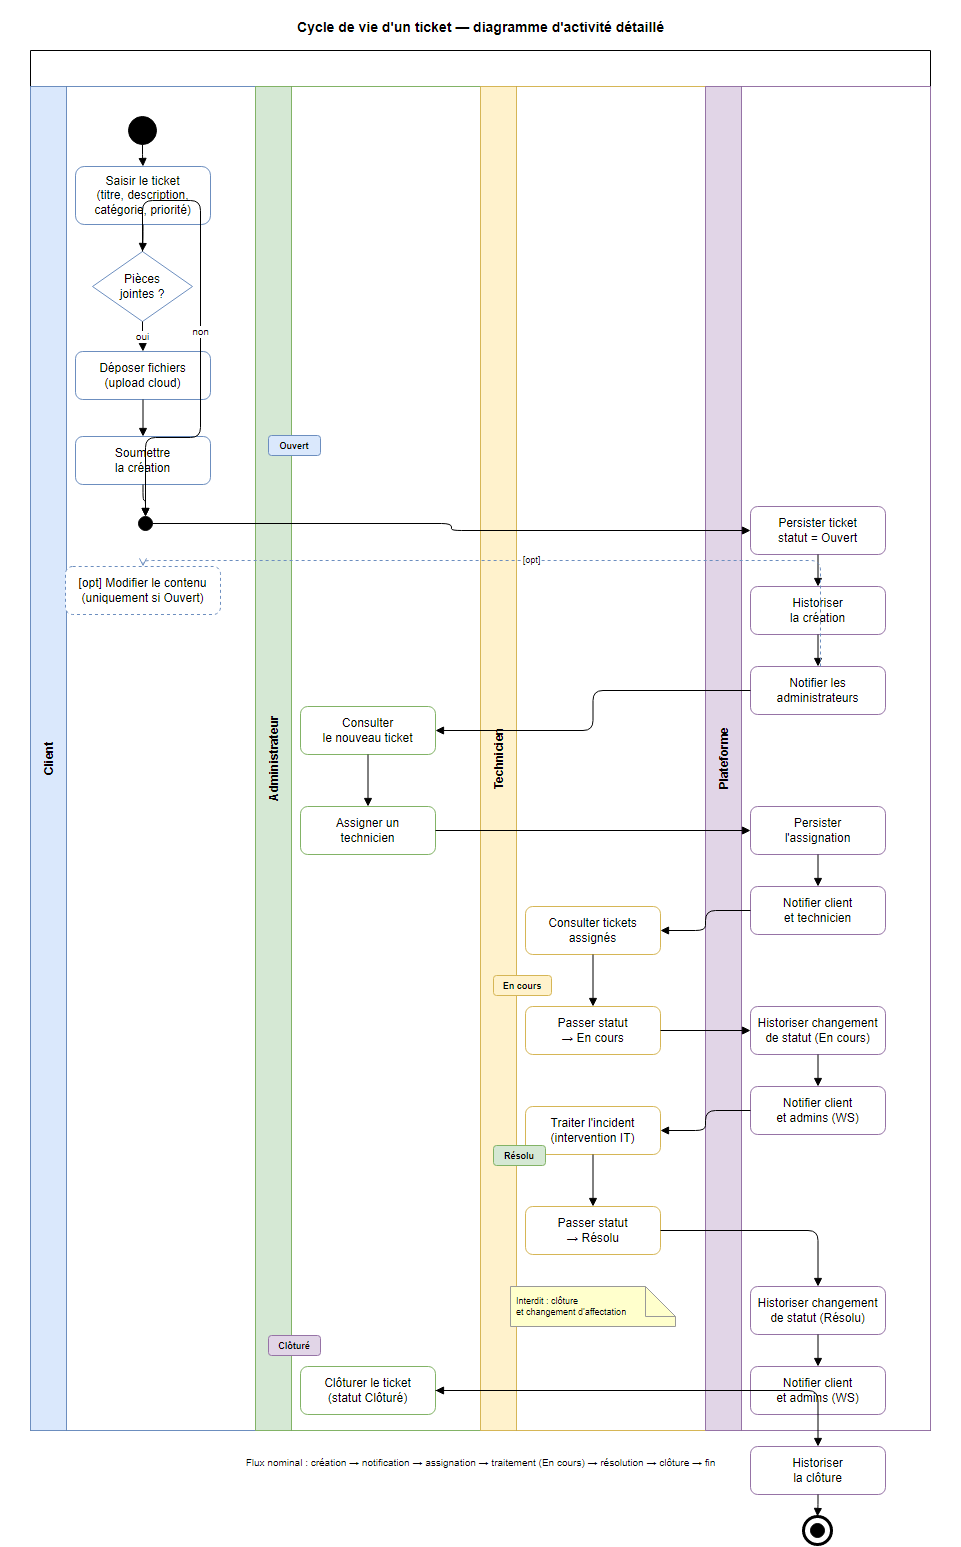
\includegraphics[width=0.95\textwidth]{img/cycle-vie-ticket-detaille.png}
    \caption{Cycle de vie d'un ticket — diagramme d'activité détaillé}
    \label{fig:cycle-vie-detaille}
\end{figure}

\paragraph{Règles métier.}
Le \textbf{client} crée le ticket (statut initial \emph{Ouvert}) et peut en
modifier le contenu tant qu'il reste ouvert. L'\textbf{administrateur} assigne
un technicien et seul lui peut passer le statut à \emph{Clôturé}. Le
\textbf{technicien} assigné fait évoluer le statut vers \emph{En cours} puis
\emph{Résolu}, sans pouvoir modifier l'affectation ni clôturer le ticket. À
chaque étape significative, la plateforme enregistre l'historique et notifie
les acteurs concernés (notifications persistantes et temps réel).

% ---------------------------------------------------------------------------
\subsubsection{Bilan}
% ---------------------------------------------------------------------------

L'adoption des patrons de conception retenus confère à \textit{TicketManager}
une structure logicielle cohérente et évolutive, traduisant au niveau
micro-architectural les principes de séparation des responsabilités, de
découplage et de réutilisabilité. Le diagramme d'activité détaillé
(figure~\ref{fig:cycle-vie-detaille}) illustre la concrétisation de ces choix
dans le cycle de vie d'un ticket, de la création à la clôture. Ainsi, la
conception en couches est complétée par un comportement métier traçable et
aligné sur les règles du domaine.
